% This template has been downloaded from:
% http://www.latextemplates.com
%
% Original author:
% Ted Pavlic (http://www.tedpavlic.com)
%
% Modified by:
% Charles Newey (http://assemblyco.de)
%----------------------------------------

% Declare document
\documentclass{article}

% Packages
\usepackage{fancyhdr} % Required for custom headers
\usepackage{lastpage} % Required to determine the last page for the footer
\usepackage{extramarks} % Required for headers and footers
\usepackage{graphicx} % Images
\usepackage{tabularx} % Tables
\usepackage[table]{xcolor} % Table colours
\usepackage[colorlinks]{hyperref} % For URLs
\usepackage[T1]{fontenc} % Support symbols like < and >
\usepackage{lmodern} % Format symbols properly

% Margins
\topmargin=-0.45in
\evensidemargin=0in
\oddsidemargin=0in
\textwidth=6.5in
\textheight=9.0in
\headsep=0.25in
\linespread{1} % Line spacing

% Other setup
\pagestyle{fancy}
\renewcommand\headrulewidth{0.4pt} % Size of the header rule
\renewcommand\footrulewidth{0.4pt} % Size of the footer rule
\setlength\parindent{0pt} % Removes all indentation from paragraphs
\renewcommand{\refname}{} % Removes bibliography title

% Set up constants
\newcommand{\address}{
\small{
	\begin{tabular}{ l}
		Department of Computer Science, \\
		Llandinam Building, \\
		Aberystwyth University, \\
		Aberystwyth, \\
		Ceredigion, \\
		SY23 3DB \\
	\end{tabular}
	}
}

% Set up the header and footer
\lhead{\doctitle}										% Top left header
\chead{\version}											% Top center head
\rhead{\firstxmark \status}								% Top right header
\lfoot{\lastxmark \qanumber}								% Bottom left footer
\cfoot{Aberystwyth University/Computer Science}			% Bottom center footer
\rfoot{Page\ \thepage\ of\ \protect\pageref{LastPage}}	% Bottom right footer

% Set up title page
\title{
	\vspace{1.2in}
	\textmd{\textbf{\doctitle}} \\
	\vspace{0.1in}\large{\textit{\today}} \\
	\vspace{0.4in}
	{\bf{\qanumber}} \\ \vspace{0.4in} % QA document number
	\version \\
	\status \\
	\vspace{0.4in}
}

\author{\authors}
\date{}


%----------------------------- UPDATE THESE FOR EACH DOCUMENT ------------------------------
\newcommand{\version}{Version: 1.2}
\newcommand{\status}{Status: Release}
\newcommand{\qanumber}{SE.10.D1}
\newcommand{\doctitle}{Group 10 Project Plan}

\newcommand{\authors}{ % Include a table for authors
	\begin{tabular}{| l | l |}
		\hline
		\bf{Contributor Name} & \bf{Role} \\
		\hline
		Daniel Clark & Project Lead \\
		\hline
		Mark Lewis & QA Manager \\
		\hline
		Charles Newey & Deputy Project Lead \& Android Developer \\
		\hline
		Martin Ferris & Android Developer \\
		\hline
		Ashley Iles & Android Developer \\
		\hline
		Kenny Packer & Android Developer \\
		\hline
		Stephen McFarlane & Deputy QA \& Web Developer \\
		\hline
		Kieran Palmer & Web Developer \\
		\hline
	\end{tabular}
	% Don't edit this
	\\ \\ \\ \\ \\ \\
	\address \vline
	\hspace{0.15in} \copyright Copyright Group 10, 2013
	% Don't edit this
}

% Make title page, ToC and other introductory elements
\begin{document}
	\maketitle
	\newpage
	\tableofcontents
	\newpage

	% Begin the actual document
	%-------------------------------------- DOCUMENT STARTS HERE ------------------------------------
	\begin{section}{INTRODUCTION}
		\begin{subsection}{Purpose of This Document}
			Purposey stuff.
		\end{subsection}
				
		\begin{subsection}{Scope}
			Scopey stuff.
		\end{subsection}
		
		\begin{subsection}{Objectives}
			\begin{itemize}
				\item{a}
				\item{b}
				\item{c}
			\end{itemize}
		\end{subsection}
	\end{section}

	\newpage
	\begin{section}{ANOTHER SECTION}
		\begin{subsection}{Introduction}
			Some text
		\end{subsection}
		
		\begin{subsection}{A Diagram}
			\begin{figure}[h!]
				\begin{center}
					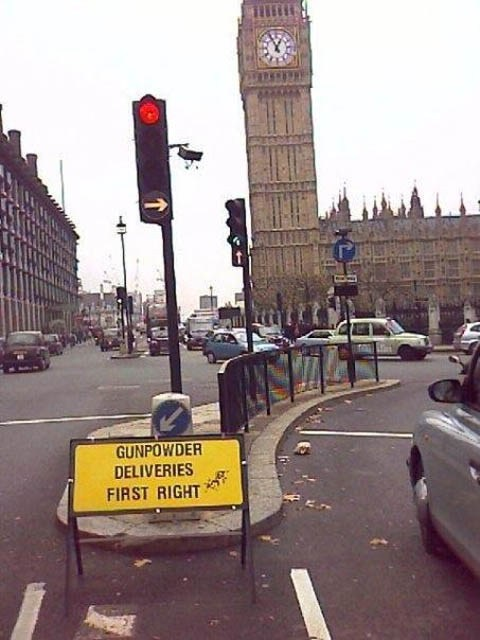
\includegraphics[height=\columnwidth]{images/test.jpg}
				\end{center}
				\caption{A caption.}
			\end{figure}
		\end{subsection}
	\end{section}
	
	\newpage
	\begin{section}{A TABLE}
		\begin{subsection}{Ongoing Tasks}
			\begin{tabularx}{\linewidth}{| p{3.5cm} | p{0.5cm} | p{0.5cm} | p{0.8cm} | X |}
				\hline
				\bf{Risk Event} & \bf{L} & \bf{M} & \bf{Risk} & \bf{Mitigation} \\
				\hline
				Team member absence & 0.6 & 0.3 & 0.18 & All team members to regularly check emails and the agreed online resources for meeting times. Being unaware of meetings is not a valid excuse. If a team member is unable to attend a meeting, the project lead (Daniel) must be notified as soon as they know they can't attend. \\
				\hline
				Project Lead absence & 0.6 & 0.5 & 0.30 & Meeting to go ahead as planned with Charlie (Deputy Project Lead) taking the meeting. \\
				\hline
				QA Manager absence & 0.6 & 0.3 & 0.18 & Meeting to go ahead as planned with Steve (Deputy QA Manager). \\
				\hline
				Unable to contact team member & 0.3 & 0.8 & 0.24 & Ensure that all team members regularly check emails and other agreed online resources, as well as checking meeting minutes so they are aware of any outstanding tasks/actions. Persistently being unreliable with result in a warning, and further action if necessary; e.g. carding or role reallocation. \\
				\hline
				Git failure & 0.3 & 1.0 & 0.3 & All work to be backed up regularly in several places in case of human error or Git failure. \\
				\hline
				Major illness or unexpected circumstances & 0.5 & 0.9 & 0.45 & Team members to be notified as soon as possible, in case any urgent tasks need to be re-assigned or completed by another team member. \\
				\hline
				Git conflict & 0.3 & 0.9 & 0.27 & All team members are to have read the information on the project wiki on Git conflicts. If a conflict is encountered, then it must be resolved immediately. If a conflict cannot be resolved easily, then an appropriate team member (Git expert/project lead) must be notified and the conflict must be resolved. Try to ensure an even task allocation, to avoid multiple team members working on the same code simultaneously. \\
				\hline
			\end{tabularx}
		\end{subsection}
	\end{section}
	
	% Include references here (edit the References.bib file)
	\nocite{LaTeXTemplate}

	% Format bibliography/refs
	\newpage
	\begin{section}{REFERENCES}
		\bibliographystyle{acm}
		\bibliography{References}
	\end{section}
	
	\vspace{1cm}
	\begin{section}{VERSION HISTORY}
		\begin{tabularx}{\linewidth}{| p{2cm} | p{2cm} | p{2cm} | X | }
			\hline
			\bf{Author} & \bf{Date} & \bf{Version} & \bf{Change made} \\
			\hline
			CCN & 07/11/2013 & 1.0 & Created template \\
			\hline
		\end{tabularx}
	\end{section}
\end{document}

%									Useful bits and pieces
%\begin{section}{section_name}								% Start section
%\end{section}												% End section
%\begin{center} \end{center}								% Center stuff
%\includegraphics[width=0.75\columnwidth]{example_figure}	% Insert image
%\pseudocode{filename}{caption}								% Insert highlighted code snippet
%\clearpage													% Clear page after section
%\url{http://www.google.com/} 								% Include URL
%\nocite{citationName}										% Cite to bibliography (but not to text)
%\cite{citationName}										% Include reference